% -*- mode: latex-mode; TeX-engine: xetex; LaTeX-command-style: (("" "SOURCE_DATE_EPOCH=0 %(PDF)%(latex) --shell-escape %S%(PDFout)")); TeX-master: "../dissertation.tex"; -*-

\chapter{Coherent Optical Creation of NaCs Molecule}
\label{ch:raman-transfer}

\section{Introduction}

\todo{emphasize general approach}

\section{Raman Transition Beyond Three-Level Model}

In an ideal three-level system, the scattering probability during a $\pi$ pulse
Raman transition can be made arbitrarily small by using a large single photon detuning.
However, in a real system, there are often other effects that increases the scattering
and may also put a lower limit on the scattering probability during the transfer.
Fig.~\ref{fig:raman-transfer-generic-raman-model} shows a generic model
for a real Raman transition demostrating some of these effects.
Additionally, other practical limitation in the system like stability of the laser power
and frequency also needs to be taken into account.

In the experiment, we find the parameter range that gives the best transfer efficiency
using numerical simulation (see section \ref{ch:raman-transfer:state-selction}).
Nevertheless, in order to develop a general approach that can be applied to other systems,
it is also important to understand the various physical mechanism that leads
to the optimal parameters.
Therefore, in this section, we will discuss some of the most important effects
on the transfer efficiency at qualitative and semiquantitative level.
Due to experimental constraint, we will assume that the single photon detuning is
much smaller than the frequency of each individual beams, i.e. $\Delta\ll\nu_1,\ \nu_2$.

\begin{figure}
  \centering
  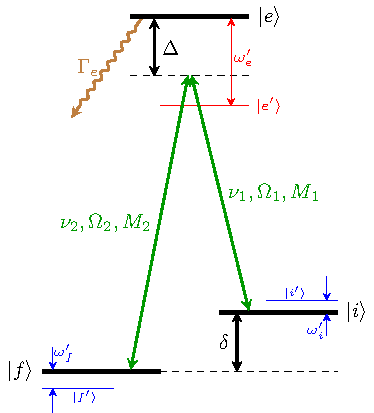
\includegraphics[width=0.6\textwidth]{figures/raman_transfer_generic_raman_model.pdf}
  \caption[Generic model for a real Raman transition]{
    Generic model for a real Raman transition.
    The initial state $|i\rangle$ and the final state $|f\rangle$
    has a energy difference $\delta$
    and are coupled by two Raman beams with frequencies and
    single photon Rabi frequencies of $\nu_1,\ \Omega_1$ and $\nu_2,\ \Omega_2$ respectively.
    The corresponding matrix elements (arbitrary unit) are $M_1$ and $M_2$.
    The Raman beams are detuned by $\Delta$ from the primary excited state $|e\rangle$,
    which has a decay rate of $\Gamma_e$.
    We also consider additional states near the initial ($|i'\rangle$),
    final ($|f'\rangle$) and intermediate excited $|e'\rangle$ states which are
    separated from the corresponding Raman transition states by $\omega'_i$,
    $\omega'_f$ and $\omega'_e$ respectively.
    Only one additional state of each kinds are included to simplify the discussion
    without loss of generality.
    \label{fig:raman-transfer-generic-raman-model}}
\end{figure}

\subsection{Additional Initial and Final States}
\label{ch:raman-transfer:extra-init-final}

First, we will discuss the effect of $|i'\rangle$ and $|f'\rangle$ states
near the initial and final states.
These states can be coupled to the excited state $|e\rangle$ by the Raman beams,
which can in tern be coupled to the initial and final states
by an off-resonance Raman transition.
The leakage is suppressed by the detuning from the Raman resonance,
i.e. $\omega'_i$ and $\omega'_f$.
This puts a limit on the Raman Rabi frequency $\Omega_R$ to be smaller
than the smallest energy gap, which in turns puts a limit on the minimum Raman transfer time.
In our experiment, the minimum energy gap comes from axial motional excitation of
the atomic initial states which is between $2\pi\times10 - 30$~kHz
depending on the trap depth used.
The typical Raman $\pi$ time we can realize is $0.5 - 5$~ms so this effect
is not a major limiting factor for our transfer efficiency.

\subsection{Additional Excited states}
\label{ch:raman-transfer:extra-ext}

\begin{figure}
  \centering
  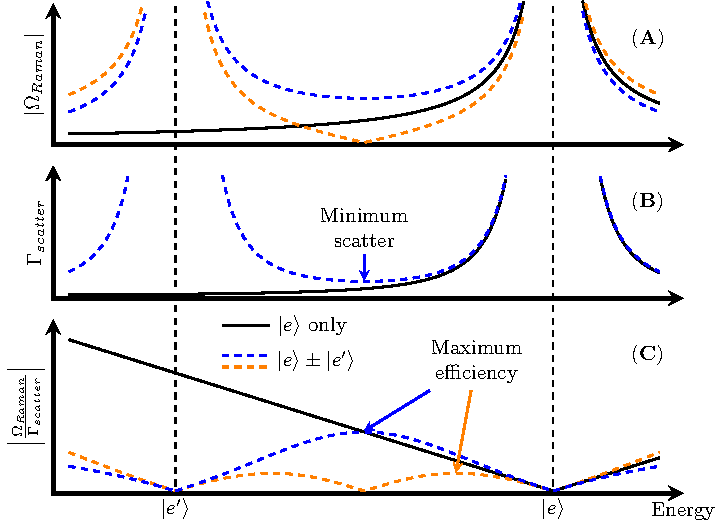
\includegraphics[width=\textwidth]{figures/raman_transfer_extra_ext_states.pdf}
  \caption[Raman transition with additional excited states]{
    Effect of additional excited states $|e'\rangle$ on the Raman transition efficiency.
    (A) Depending on the sign of the coupling, there could be constructive (blue)
    or destructive (orange) interference on the Raman Rabi frequency $\Omega_{Raman}$.
    (B) Increased scattering rate $\Gamma_{scatter}$ caused by $|e'\rangle$ with a minimal
    between the two states.
    (C) Optimal detunine exists between the two states with maximum transfer efficiency
    corresponds to a fraction of the state spacing.
    \label{fig:raman-transfer-extra-ext-states}}
\end{figure}

Next, we will consider the effect of the $|e'\rangle$ state near the excited intermediate state.
These states can be coupled to the ground states, both $|i\rangle$ and $|f\rangle$,
by the Raman beams and can cause a change in both the Raman Rabi frequency
and the scattering rate.
The total Raman Rabi frequency (Fig.~\ref{fig:raman-transfer-extra-ext-states}A) is,
\[
  \Omega_{Raman}=\frac{\Omega_1\Omega_2}{2\Delta}+\frac{\Omega'_1\Omega'_2}{2(\Delta-\omega'_e)}
\]
where $\Omega'_1$ and $\Omega'_2$ are the single photon Rabi frequencies coupling $|e'\rangle$
to $|i\rangle$ and $|f\rangle$ respectively.
Depending on whether $\Omega'_1\Omega'_2$ has the same (orange line)
or different (blue line) sign as $\Omega_1\Omega_2$, the total Raman Rabi frequency
may be cancelled or enhanced between the two excited states.
On the other hand, the total scattering rate (Fig.~\ref{fig:raman-transfer-extra-ext-states}B)
is almost always increased due to the additional state, creating a local minimum
between the excited states.
Combining the two effects, the ratio between the Raman Rabi frequency and
the scattering rate, which determines the transfer efficiency, always have local maximum
between the excited states (Fig.~\ref{fig:raman-transfer-extra-ext-states}C).

Despite the difference in the position and value of the maximum for different
$|e'\rangle$ parameters, we can summarize the effect on the transfer efficiency
as a limit on the maximum detuning $\Delta_{max}$ to a fraction of the spacing
between the excited states ($\omega'_e$).
As an example, the blue and orange maxima in Fig.~\ref{fig:raman-transfer-extra-ext-states}C
corresponds to a limit on single photon detuning of $0.5\omega'_e$ and $0.15\omega'_e$.
As one would expected, a larger excited state spacing usually result in
a larger detuning limit and a better transfer efficiency.

Summarizing the effect of additional excited state as a single number $\Delta_{max}$ allows
us to keep using the equation for Raman transition with minor corrections
and makes it easier to compare different state selection and transition schemes.
It is also worth noting that although only one additional excited state $|e'\rangle$
is considered here, this result can be generalized when more excited states are taken into account
as well. These states introduces additional smooth variation in both the Raman Rabi frequency
and scattering rate and the effects on the final transition efficiency can be similarly
treated as a change in the maximum detuning.

\subsection{Cross Coupling Between Light Addressing Initial and Final States}
\label{ch:raman-transfer:cross-couple}

Due to the small energy separation between the initial and final state $\delta$,
the cross coupling of the laser addressing the initial/final state on the final/initial state
is another important effect in our experiment.
Without the cross coupling, the total off resonance scattering rate for
the initial and the final states is
\[
  \Gamma_{scatter0}=\frac{\Gamma_e\left(\Omega_1^2+\Omega_2^2\right)}{4\Delta^2}
\]
For a given Raman Rabi frequency $\Omega_{Raman}\propto\Omega_1\Omega_2$, this is
minimized when $\Omega_1=\Omega_2$.\todo{\cite{}}

When cross coupling is taken into account, however, the total scattering rate becomes,
\footnote{Here we assume that the matrix elements are the same for the two beams.
  This is the case when the two beams have the same polarization as in our experiment.
  This effect can be minimized or eliminated by selecting different polarizations for the
  two laser frequencies that does not couple to the other initial/final state.
  This would also require choosing an excited state with the same or lower angular momentum
  as the ground states in order to avoid cross coupling to different excited states.}
\begin{align}
  \Gamma_{scatter}=&\frac{\Gamma_e\Omega_1^2}{4M_1^2}\left(\frac{M_1^2}{\Delta^2}+\frac{M_2^2}{(\Delta+\delta)^2}\right)+\frac{\Gamma_e\Omega_2^2}{4M_2^2}\left(\frac{M_2^2}{\Delta^2}+\frac{M_1^2}{(\Delta-\delta)^2}\right)\\
  \propto&\frac{\Gamma_eP_1}{4}\left(\frac{M_1^2}{\Delta^2}+\frac{M_2^2}{(\Delta+\delta)^2}\right)+\frac{\Gamma_eP_2}{4}\left(\frac{M_2^2}{\Delta^2}+\frac{M_1^2}{(\Delta-\delta)^2}\right)
\end{align}
where $P_{1,2}\propto\Omega_{1,2}^2/M_{1,2}^2$ are the powers of the laser beams 1 and 2.
When $\delta\ll\Delta$ such as our experiment,
\begin{align*}
  \Gamma_{scatter}\approx&\frac{\Gamma_e\left(M_1^2+M_2^2\right)}{4\Delta^2}\left(\frac{\Omega_1^2}{M_1^2}+\frac{\Omega_2^2}{M_2^2}\right)\\
  \propto&\frac{\Gamma_e\left(M_1^2+M_2^2\right)}{4\Delta^2}\left(P_1+P_2\right)
\end{align*}
For a given Raman Rabi frequency $\Omega_{Raman}\propto\Omega_1\Omega_2\propto\sqrt{P_1P_2}$,
this is minimized when $P_1=P_2$.
Hence, due to the strong cross coupling, we need to use the same power in both Raman beams
rather than adjusting the powers to match their single photon Rabi frequencies.

Moreover, at the minimum scattering rate, we have $\Omega_2=\Omega_1M_2/M_1$
and the ratio between Raman Rabi frequency and scattering rate is,
\begin{align*}
  \frac{\Omega_{Raman}}{\Gamma_{scatter}}=&\frac{\Omega_1\Omega_2}{2\Delta}\frac{4\Delta^2}{\Gamma_e\left(M_1^2+M_2^2\right)}\left/\left(\frac{\Omega_1^2}{M_1^2}+\frac{\Omega_2^2}{M_2^2}\right)\right.\\
  =&\frac{2\Delta\Omega_1\Omega_2}{\Gamma_e\left(M_1^2+M_2^2\right)}\left/\left(\frac{\Omega_1^2}{M_1^2}+\frac{\Omega_2^2}{M_2^2}\right)\right.\\
  =&\frac{\Delta\Omega_1^2M_2}{\Gamma_eM_1\left(M_1^2+M_2^2\right)}\frac{M_1^2}{\Omega_1^2}\\
  =&\frac{\Delta}{\Gamma_e}\frac{M_1M_2}{M_1^2+M_2^2}
\end{align*}
Therefore, for a given excited state linewidth $\Gamma_e$
and maximum detuning (section \ref{ch:raman-transfer:extra-ext}) the transfer efficiency
maximizes for the smallest $M_1M_2/(M_1^2+M_2^2)$ which happens when the ratio
$M_1/M_2$ is the closest to $1$.

The light shift of the Raman resonance is similarly affected by the cross coupling.
The differential light shift between the initial and the final state determines
the resonance fluctuation as a function of light intensity fluctuation.
The ration between the light shift and the Raman Rabi frequency, i.e. line width,
determines the stability requirement of our laser indensity.
With cross coupling, the differential shift is (assuming $\delta\ll\Delta$),
\begin{align*}
  \Delta\delta\approx&\frac{\Omega_1^2}{4\Delta}-\frac{\Omega_1^2M_2^2}{4\Delta M_1^2}-\frac{\Omega_2^2}{4\Delta}+\frac{\Omega_2^2M_1^2}{4\Delta M_2^2}\\
  =&\frac{M_1^2-M_2^2}{4\Delta}\left(\frac{\Omega_1^2}{M_1^2}+\frac{\Omega_2^2}{M_2^2}\right)\\
  \propto&\frac{M_1^2-M_2^2}{4\Delta}\left(P_1+P_2\right)
\end{align*}
which is also minimized when $P_1=P_2$ at a given Raman Rabi frequency.

The ratio with the Raman Rabi frequency is,
\begin{align*}
  \frac{\Delta\delta}{\Omega_{Raman}}\approx&\frac{M_1^2-M_2^2}{4\Delta}\left(\frac{\Omega_1^2}{M_1^2}+\frac{\Omega_2^2}{M_2^2}\right)\frac{2\Delta}{\Omega_1\Omega_2}\\
  =&\frac{M_1^2-M_2^2}{2\Omega_1\Omega_2}\left(\frac{\Omega_1^2}{M_1^2}+\frac{\Omega_2^2}{M_2^2}\right)\\
  =&\frac{M_1^2-M_2^2}{M_1M_2}
\end{align*}
the absolute value of which is also minimized when the ratio $M_1/M_2$ is the closest to $1$.

Due to the coupling strength difference, we have $M_2\gg M_1$ in our experiment, which means,
\begin{align*}
  \left|\frac{\Delta\delta}{\Omega_{Raman}}\right|\approx&\frac{M_2}{M_1}
\end{align*}
In order to keep the resonance stable within the linewidth of the Raman resonance,
i.e. $\Omega_{Raman}$, we need to maintain a relative stability of $\Delta\delta$,
therefore relative stability of the laser power to better than $M_1/M_2$.

\section{Raman Transfer versus STIRAP}

An alternative method often used to create and prepare the internal states of ultracold molecule
is stimulated Raman adiabatic passage (STIRAP)\todo{\cite{}}.
Compared to Raman transition, which uses detuning from the excited state
to reduce scattering during the transfer, STIRAP relies on a superposition between
the initial and final state as a dark state to achieve the same goal.
The dark state in STIRAP is created due to a destructive interference of transition
from the initial and final state to the excited state.

Similar to Raman transfer, STIRAP in an ideal three-level system can achieve
full coherent transfer with arbitrarily small scattering probability
when given unlimited time and power budget.
However, in reality, states and coupling that exist outside the ideal three-level system
always cause a non-zero probability of scattering loss
(see Fig.~\ref{fig:raman-transfer-generic-stirap-model}).
In this section, we will apply the approach we took for Raman transition to STIRAP.
We will then compare the loss caused by different practical limitations
and discuss which approach should be taken under certain circumstance.

\begin{figure}
  \centering
  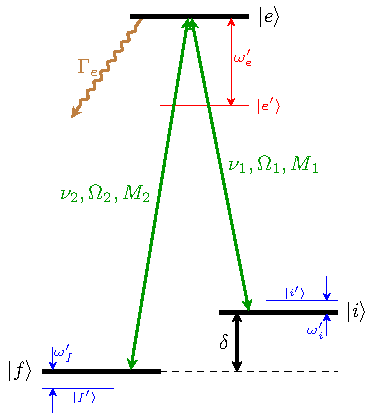
\includegraphics[width=0.6\textwidth]{figures/raman_transfer_generic_stirap_model.pdf}
  \caption[Generic model for a real STIRAP]{
    Generic model for a real STIRAP similar to Fig.~\ref{fig:raman-transfer-generic-raman-model}.
    Differences are that the two beams are now on resonant with $|e\rangle$
    and the $\Omega_1$ and $\Omega_2$ now represent the maximum single photon Rabi frequency
    during the STIRAP pulse.
    \label{fig:raman-transfer-generic-stirap-model}}
\end{figure}

\subsection{Additional Initial and Final States}

Similar to Raman transition (section \ref{ch:raman-transfer:extra-init-final}),
the additional initial and final states causes potential leakage out of the three-level system.
This limits the minimum time of the transfer in a way similar to that of Raman transition.

\subsection{Additional Excited states}

\subsection{Cross Coupling Between Light Addressing Initial and Final States}

\subsection{Conclusion}

\todo{mention use of tweezer as Raman}

\section{States Selection}
\label{ch:raman-transfer:state-selction}

(Differential Light Shift)
(Scattering)

\subsection{Excited State Selection}

\subsection{Ground States Selection}

\subsubsection{Final Molecular State}

\subsubsection{Initial Atomic State}

\section{Raman Transfer Results}

\subsection{Scaling of Raman Transition Parameters}

\todo{mention significance of atomic scattering}
